\documentclass[11pt]{article}

% ---------- Packages ----------
\usepackage[utf8]{inputenc}
\usepackage[T1]{fontenc}
\usepackage{amsmath, amssymb, amsthm}
\usepackage{geometry}
\usepackage{booktabs}
\usepackage{array}
\usepackage{multirow}
\usepackage{xcolor}
\usepackage{enumitem}
\usepackage{hyperref}
\usepackage{graphicx}
\usepackage{float}
\usepackage{tikz}
\usetikzlibrary{arrows.meta, positioning, shapes.geometric}
\graphicspath{{images/}{./}}

\geometry{a4paper, margin=1in}
\hypersetup{
    colorlinks=true,
    linkcolor=blue!60!black,
    urlcolor=blue!60!black,
    citecolor=blue!60!black
}

% ---------- Custom commands ----------
\newcommand{\OL}{\mathit{OL}}
\newcommand{\OW}{\mathit{OW}}
\newcommand{\OH}{\mathit{OH}}
\newcommand{\WB}{\mathit{WB}}
\newcommand{\TW}{\mathit{TW}}
\newcommand{\given}{\,\vert\,}
\newcommand{\Rtrim}{R_{\text{trim}}}
\newcommand{\NLL}{\text{NLL}}

\theoremstyle{definition}
\newtheorem{remark}{Remark}

\title{\textbf{Vehicle-Type--Specific Gaussian Models for\\ 3D Car Reconstruction and Classification}\\[4pt]
\large A Technical Walkthrough: From a Single Average Model to a Type-Aware Pipeline}
\author{Project Report}
\date{\today}

\begin{document}
\maketitle

\begin{abstract}
\noindent This report documents the evolution of a 3D vehicle reconstruction pipeline. The original system used a \emph{single}, type-agnostic statistical model that rendered every vehicle as a population-average shape. The redesigned system maintains \emph{four} per-type Gaussian shape models and four parametric mesh templates (sedan, SUV, truck, van). Given a sparse 3D point cloud and predicted exterior dimensions, the new pipeline fits all four type-specific models, scores each by how well it explains the points, and both renders the best-fitting shape and classifies the vehicle by which model wins. We formalise the conditional-Gaussian shape model, trace exactly how the recovered parameters drive the mesh rendering, derive the selection score, and document the four engineering challenges whose solutions took classification accuracy from $1/3$ to $3/3$ on the labelled sample set. We also compare four interchangeable rendering back-ends --- a single procedural template, four per-type parametric polygons, a rigidly-stretched photoreal \texttt{.glb}, and a parametric Kenney-kit reconstruction --- and the trade-off they expose between visual realism and faithfulness to the predicted parameters.
\end{abstract}

\tableofcontents
\vspace{1em}
\hrule
\vspace{1em}

% =====================================================================
\section{Inputs and Parameterisation}
% =====================================================================

Each detected vehicle is described by two inputs:
\begin{enumerate}[leftmargin=2em]
    \item A set of \textbf{predicted exterior dimensions} produced by an upstream detector.
    \item A \textbf{sparse 3D point cloud} of 16--19 semantic keypoints.
\end{enumerate}

The vehicle is modelled using 11 scalar parameters, partitioned into two groups: the \emph{known} (observed) exterior dimensions $b$, and the \emph{unknown} interior/proportion parameters $a$ that must be predicted.

\begin{equation}
b = (\OW,\ \WB,\ \OH,\ \OL), \qquad
a = (A,\ C,\ D,\ E,\ F,\ G,\ \TW).
\end{equation}

\begin{table}[h]
\centering
\begin{tabular}{cl}
\toprule
\textbf{Symbol} & \textbf{Meaning} \\
\midrule
$\OL,\OW,\OH$ & overall length, width, height \\
$\WB$ & wheelbase (conditioning only) \\
$A$ & front bumper to base of windshield \\
$C$ & side-window height \\
$D$ & door height (below the window) \\
$E$ & greenhouse (roof) width / inset \\
$F,\ G$ & front and rear overhang (axle offsets) \\
$\TW$ & mean track width \\
\bottomrule
\end{tabular}
\caption{The 11 vehicle parameters.}
\end{table}

\noindent Three quantities are derived deterministically from the above:
\begin{equation}
r_{\text{tire}} = \OH - C - D, \qquad
w_{\text{tire}} = \OW - \TW, \qquad
h_{\text{belt}} = \OH - C.
\end{equation}

% =====================================================================
\section{The Original Single-Model Pipeline (Before)}
% =====================================================================

\subsection{The common Gaussian conditional model}

A \emph{single} multivariate Gaussian was fitted over all vehicles in the pooled 2011--2023 dataset, jointly modelling the known dimensions $b$ and the unknown proportions $a$:
\begin{equation}
\begin{pmatrix} a \\ b \end{pmatrix}
\sim \mathcal{N}\!\left(
\begin{pmatrix} \mu_a \\ \mu_b \end{pmatrix},\
\begin{pmatrix} \Sigma_{aa} & \Sigma_{ab} \\ \Sigma_{ba} & \Sigma_{bb} \end{pmatrix}
\right).
\label{eq:joint}
\end{equation}

The symbol $\sim \mathcal{N}(\mu,\Sigma)$ reads ``is distributed as a multivariate Gaussian with mean vector $\mu$ and covariance matrix $\Sigma$.'' The covariance blocks have the following sizes and meaning:
\begin{center}
\begin{tabular}{ccl}
\toprule
\textbf{Block} & \textbf{Size} & \textbf{Meaning} \\
\midrule
$\Sigma_{aa}$ & $7\times7$ & co-variation among hidden parameters \\
$\Sigma_{bb}$ & $4\times4$ & co-variation among exterior dimensions \\
$\Sigma_{ab}$ & $7\times4$ & cross-covariance (the key prediction block) \\
$\Sigma_{ba}$ & $4\times7$ & transpose of $\Sigma_{ab}$ \\
\bottomrule
\end{tabular}
\end{center}

\paragraph{Building the covariance matrix.} Given a dataset of $n$ vehicles, each stacked into an 11-vector $x^{(k)} = (a^{(k)}, b^{(k)})$:
\begin{equation}
\mu = \frac{1}{n}\sum_{k=1}^{n} x^{(k)}, \qquad
\Sigma = \frac{1}{n-1}\sum_{k=1}^{n} (x^{(k)} - \mu)(x^{(k)} - \mu)^{\top},
\end{equation}
then partition $\Sigma$ into the four blocks according to which indices belong to $a$ and which to $b$.

\paragraph{Predicting the hidden parameters.} Given an observed $b$, the missing parameters were predicted by the Gaussian \emph{conditional mean}:
\begin{equation}
\hat{a} = \mathbb{E}[a \given b] = \mu_a + \Sigma_{ab}\,\Sigma_{bb}^{-1}(b - \mu_b).
\label{eq:cond}
\end{equation}

This is the exact, closed-form posterior mean when both variables are jointly Gaussian. Reading it term by term:
\begin{itemize}[leftmargin=2em]
    \item $(b - \mu_b)$ --- how far this vehicle's exterior deviates from the average;
    \item $\Sigma_{bb}^{-1}$ --- normalises that deviation by the typical spread of exterior dimensions;
    \item $\Sigma_{ab}$ --- projects the normalised deviation into the hidden-parameter space using learned correlations;
    \item $\mu_a$ --- the population baseline to which the data-driven correction is added.
\end{itemize}

\subsection{Wireframe geometry and the height levels}

The recovered parameters were turned into a fixed wireframe mesh (a lower body box, a greenhouse with sloped windshield and rear window, a flat roof, and four tire cylinders). The three defining vertical levels are:
\begin{equation}
y_{\text{sill}} = \OH - C - D, \qquad
y_{\text{belt}} = \OH - C, \qquad
y_{\text{roof}} = \OH.
\label{eq:heights}
\end{equation}

\subsection{Rigid fitting to the point cloud}

The mesh \emph{shape} was fixed; only its \emph{pose} was optimised. Let $P = \{p_i\}_{i=1}^N$ be the (centred, cm-scaled) point cloud and $S$ the mesh surface. With a single global translation $t \in \mathbb{R}^3$ and a heading rotation $R(\theta)$ about the vertical axis, each point is mapped into the model frame:
\begin{equation}
q_i = R(\theta)^{\top}(p_i - t),
\end{equation}
and its unsigned distance to the nearest surface element is computed:
\begin{equation}
d_i(t,\theta) = \min_{s \in S}\ \text{dist}\!\left(R(\theta)^{\top}(p_i - t),\ s\right).
\label{eq:dist}
\end{equation}
For a quad face the distance is the in-plane projection distance when the projection falls inside the quad, and the nearest-edge distance otherwise. The pose minimises the weighted mean squared distance,
\begin{equation}
\mathcal{L}(t,\theta) = \frac{1}{N}\sum_{i=1}^{N} w_i\, d_i(t,\theta)^2,
\label{eq:loss}
\end{equation}
using 50 iterations of RMSProp (autograd through the distance functions), with $w_i$ up-weighting the tire term for ground-level points.

\begin{remark}[Translation vs.\ rotation]
The translation $t$ is a \emph{single global vector} subtracted from every point identically; it is order- and distance-preserving and can never turn a front point into a rear point. Only the rotation $R(\theta)$ can flip orientation. A $180^\circ$ heading error causes front keypoints to be matched against rear mesh surfaces in Eq.~\eqref{eq:dist} --- the root of Challenge~2.
\end{remark}

\subsection{Limitation of the original pipeline}
Because a single Gaussian and a single template were used, the rendered shape was always the population average --- a fastback/SUV-like silhouette. The system had no notion of vehicle type and could represent neither a pickup's bed nor a sedan's trunk.

% =====================================================================
\section{The Multi-Model Redesign (Now)}
% =====================================================================

The redesign keeps the same conditional-Gaussian machinery but \emph{instantiates it per type} and adds a model-selection step. No new mathematical machinery is introduced.

\begin{center}
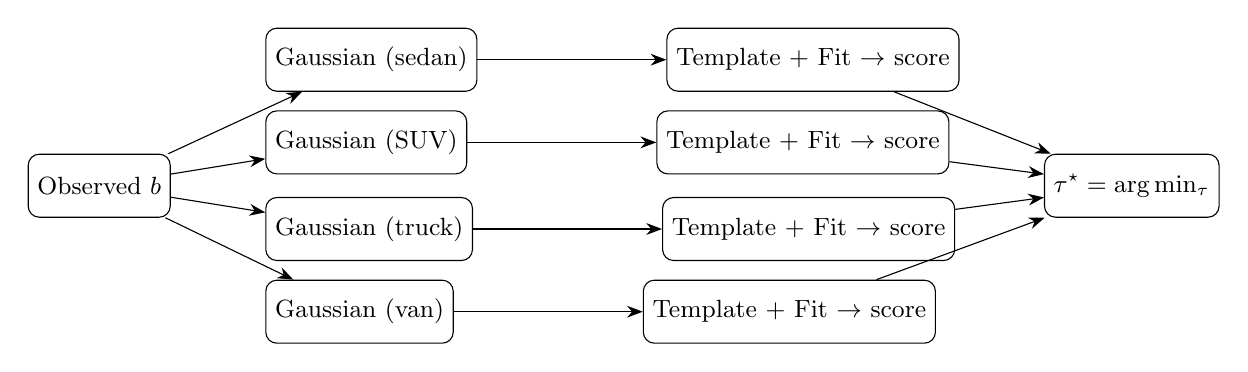
\begin{tikzpicture}[
    node distance=0.45cm and 1.2cm,
    box/.style={draw, rounded corners, align=center, minimum height=0.8cm, font=\small},
    arr/.style={-{Stealth[length=2mm]}}
]
\node[box] (in) {Observed $b$};
\node[box, right=of in, yshift=1.6cm] (g1) {Gaussian (sedan)};
\node[box, right=of in, yshift=0.55cm] (g2) {Gaussian (SUV)};
\node[box, right=of in, yshift=-0.55cm] (g3) {Gaussian (truck)};
\node[box, right=of in, yshift=-1.6cm] (g4) {Gaussian (van)};
\node[box, right=2.4cm of g1] (s1) {Template + Fit $\rightarrow$ score};
\node[box, right=2.4cm of g2] (s2) {Template + Fit $\rightarrow$ score};
\node[box, right=2.4cm of g3] (s3) {Template + Fit $\rightarrow$ score};
\node[box, right=2.4cm of g4] (s4) {Template + Fit $\rightarrow$ score};
\node[box, right=1.2cm of s2, yshift=-0.55cm] (out) {$\tau^\star = \arg\min_\tau$};

\foreach \g in {g1,g2,g3,g4} \draw[arr] (in) -- (\g);
\draw[arr] (g1) -- (s1);
\draw[arr] (g2) -- (s2);
\draw[arr] (g3) -- (s3);
\draw[arr] (g4) -- (s4);
\foreach \s in {s1,s2,s3,s4} \draw[arr] (\s) -- (out);
\end{tikzpicture}
\end{center}

\subsection{Stage 1 --- per-type Gaussian models}

Four separate Gaussians are trained, one per category $\tau \in \{\text{sedan},\text{suv},\text{truck},\text{van}\}$, each only on that category's rows. Conditioning on the same observed $b$ now yields a \emph{type-specific} prediction:
\begin{equation}
\hat{a}^{(\tau)} = \mu_a^{(\tau)} + \Sigma_{ab}^{(\tau)}\big(\Sigma_{bb}^{(\tau)}\big)^{-1}\!\big(b - \mu_b^{(\tau)}\big).
\label{eq:condtau}
\end{equation}
The same $b$ produces four geometrically distinct predictions because each model learned different average proportions and correlations from its own data (e.g.\ a truck Gaussian predicts a short greenhouse and long bed; a sedan Gaussian predicts a lower roofline and a trunk gap).

\subsection{Stage 2 --- per-type geometry templates}

The single template is replaced by four, all built from one shared ``model-car'' recipe (the Sketch-up / Model-Car-Vertices construction from the design doc). Every type reuses an identical \emph{tapered nose} (an inset grille panel chamfered out to full width, faces 1--5), an identical \emph{lower body} (the doors, beltline down to sill) and an identical \emph{underbody}; only the structure \emph{above the beltline} changes per type. This keeps the four meshes watertight and mutually consistent while letting each express its own greenhouse, trunk or bed. The greenhouse is laterally inset by $(\OW-E)/2$, so the recovered $E$ narrows the cabin directly.

\begin{table}[h]
\centering
\begin{tabular}{p{1.6cm} p{8.3cm} c}
\toprule
\textbf{Type} & \textbf{Structure above the beltline} & \textbf{Quads} \\
\midrule
SUV   & two-box; inset greenhouse, rear glass straight to the beltline & 14 \\
Van   & two-box, taller; upright windshield, roof carried to the tail & 14 \\
Sedan & three-box; inset cabin, sloped rear glass, lower full-width trunk deck (with C-pillar ``sail'' quads) & 19 \\
Truck & full-width cab + open bed (bed floor, side rails, tailgate) & 18 \\
\bottomrule
\end{tabular}
\caption{The four parametric templates (\texttt{car\_models\_core\_new}). The fitting loss is generic over the quad list, so differing face counts need no special casing.}
\end{table}

\subsection{How the recovered parameters drive the rendering}

Every mesh vertex is a deterministic function of the 11 parameters. The key insight is that the outer bounding box comes from $b$, but \emph{almost everything inside it} comes from the predicted $\hat{a}^{(\tau)}$ --- which is precisely why four different $\hat{a}^{(\tau)}$ over the same $b$ yield four discriminable shapes.

\begin{table}[h]
\centering
\renewcommand{\arraystretch}{1.15}
\begin{tabular}{>{\ttfamily}c c p{8.5cm}}
\toprule
\textbf{Param} & \textbf{Source} & \textbf{Used to build} \\
\midrule
OL & $b$ & body length, all $z$-profile positions, rear bumper \\
OW & $b$ & body width, tire width $(\OW-\TW)$ \\
OH & $b$ & $y_{\text{roof}}$; feeds $y_{\text{belt}}, y_{\text{sill}}$; tire radius \\
WB & $b$ & rear axle position $(F+\WB)$ \\
A  & $\hat{a}^{(\tau)}$ & windshield-base $z$, roofline start $A+\tfrac{2}{10}(\OL-A)$ \\
C  & $\hat{a}^{(\tau)}$ & $y_{\text{belt}}=\OH-C$, $y_{\text{sill}}=\OH-C-D$, window height, tire radius \\
D  & $\hat{a}^{(\tau)}$ & $y_{\text{sill}}=\OH-C-D$, tire radius \\
E  & $\hat{a}^{(\tau)}$ & greenhouse lateral inset (\texttt{off}), roof narrowing \\
F  & $\hat{a}^{(\tau)}$ & front axle $z$-position, roofline anchor \\
G  & $\hat{a}^{(\tau)}$ & rear overhang, rear-axle confirmation $G=\OL-F-\WB$ \\
TW & $\hat{a}^{(\tau)}$ & tire lateral positions $(\pm \TW/2)$, tire width $(\OW-\TW)$ \\
\bottomrule
\end{tabular}
\caption{Parameter-to-geometry map. $b$ sets the outer box; $\hat{a}^{(\tau)}$ sets the interior.}
\end{table}

\subsection{Best-fit selection}

All four type models are built and fitted; the type whose fitted shape best explains the points is both rendered and taken as the predicted class:
\begin{equation}
\tau^\star = \arg\min_\tau\ \text{score}(\tau).
\label{eq:argmin}
\end{equation}
Because the exterior box $(\OW,\OH,\OL,\WB)$ is identical across the four candidates, the comparison isolates the internal silhouette --- exactly where the categories differ.

% =====================================================================
\section{Mathematical Formulation of the Selection Score}
% =====================================================================

The score combines a robust geometric residual with a statistical prior on the exterior dimensions.

\subsection{Robust (trimmed) geometric residual}

Let $B \subseteq P$ be the body points (above a small height threshold) and $d_{(1)} \le d_{(2)} \le \cdots \le d_{(M)}$ the sorted point--surface distances at the fitted pose. Discarding the worst fraction $\rho$ of points yields:
\begin{equation}
\Rtrim(\tau) = \frac{1}{K}\sum_{i=1}^{K} d_{(i)}^2, \qquad K = \big\lfloor (1-\rho)\,M \big\rfloor,\quad \rho = 0.2.
\label{eq:rtrim}
\end{equation}
This is the mean squared distance of the $80\%$ best-fitting body points --- an outlier-resistant estimator that removes accessory keypoints (cargo racks, antennas) that conform to no template.

\subsection{Exterior-dimension prior}

Each type's Gaussian induces a \emph{marginal} over the exterior dimensions, obtained by integrating out the unobserved $a$:
\begin{equation}
b \given \tau \sim \mathcal{N}\!\big(\mu_b^{(\tau)},\ \Sigma_{bb}^{(\tau)}\big).
\end{equation}
The marginal is the correct likelihood to use because $a$ is never observed, and substituting the predicted $\hat{a}^{(\tau)}$ would be circular (it already assumes type $\tau$). Its negative log-likelihood (dropping the type-independent $\tfrac{d}{2}\log 2\pi$ constant) is:
\begin{equation}
\NLL(\tau) = \underbrace{\tfrac{1}{2}\big(b-\mu_b^{(\tau)}\big)^{\top}\big(\Sigma_{bb}^{(\tau)}\big)^{-1}\big(b-\mu_b^{(\tau)}\big)}_{\text{Mahalanobis distance}}
+ \underbrace{\tfrac{1}{2}\log\big|\Sigma_{bb}^{(\tau)}\big|}_{\text{log-determinant}}.
\label{eq:nll}
\end{equation}

\begin{itemize}[leftmargin=2em]
    \item \textbf{Mahalanobis term:} the statistical distance of $b$ from type $\tau$'s typical dimensions, normalised by the type's spread. A $5.8$\,m vehicle scores low against the truck mean and devastatingly high against the sedan mean.
    \item \textbf{Log-determinant term:} a normalisation that penalises broad, diffuse distributions. Without it, a type with huge variance would win by accepting almost any vehicle; the log-det makes a tight, specific distribution score lower when the dimensions genuinely match.
\end{itemize}

\subsection{Combined score}

\begin{equation}
\boxed{\ \text{score}(\tau) = \Rtrim(\tau) + \lambda\,\NLL(\tau)\ }
\label{eq:score}
\end{equation}
with $\lambda$ balancing geometric fit against the dimensional prior. The first term answers \emph{``does this shape match the points?''}; the second answers \emph{``are these dimensions typical of this type?''} Structurally this is a Bayesian model-selection criterion: $\Rtrim$ acts as the likelihood, $\NLL$ as the prior, and $\tau^\star$ is the MAP decision.

% =====================================================================
\section{Type-Selection Algorithm}
% =====================================================================

\begin{table}[h]
\centering
\begin{tabular}{p{0.92\textwidth}}
\toprule
\textbf{Algorithm 1:} Type selection for one vehicle \\
\midrule
\textbf{Require:} point cloud $P$, exterior dims $b=(\OW,\WB,\OH,\OL)$, heading guess $\theta_0$ \\[2pt]
\textbf{for} $\tau \in \{\text{sedan},\text{suv},\text{truck},\text{van}\}$ \textbf{do} \\
\quad $\hat{a}^{(\tau)} \leftarrow \mu_a^{(\tau)} + \Sigma_{ab}^{(\tau)}(\Sigma_{bb}^{(\tau)})^{-1}(b-\mu_b^{(\tau)})$ \hfill $\triangleright$ Eq.~\eqref{eq:condtau} \\
\quad build mesh $S^{(\tau)}$ from $(\hat{a}^{(\tau)}, b)$ \\
\quad \textbf{for} $\delta \in \{0^\circ, 180^\circ\}$ \textbf{do} \hfill $\triangleright$ heading multi-start \\
\quad\quad $(t,\theta) \leftarrow \arg\min \mathcal{L}$ from $\theta_0 + \delta$ \hfill $\triangleright$ Eq.~\eqref{eq:loss} \\
\quad\quad keep the start with the smaller $\Rtrim$ \hfill $\triangleright$ Eq.~\eqref{eq:rtrim} \\
\quad \textbf{end for} \\
\quad $\text{score}(\tau) \leftarrow \Rtrim(\tau) + \lambda\,\NLL(\tau)$ \hfill $\triangleright$ Eqs.~\eqref{eq:nll}--\eqref{eq:score} \\
\textbf{end for} \\
\textbf{return} $\tau^\star = \arg\min_\tau \text{score}(\tau)$ \\
\bottomrule
\end{tabular}
\end{table}

% =====================================================================
\section{Rendering Back-Ends: Four Display Strategies}
% =====================================================================

The type decision and the fitted pose are produced once by the selection core
(\texttt{car\_models\_core}); \emph{what is drawn at that pose} is a separate
choice. Four interchangeable renderers were built, trading off visual realism
against how many of the eleven predicted parameters actually deform the displayed
mesh. This is the central tension: \textbf{the more photoreal the display, the
fewer of the predicted parameters it can honour.}

\paragraph{Shared technology stack.} All four use the same plumbing: a
\textbf{PyQt5} \texttt{QOpenGLWidget} for the window and GL context,
\textbf{PyOpenGL} (\texttt{OpenGL.GL/GLU/GLUT}) for immediate-mode drawing,
\textbf{NumPy}/\textbf{pandas} for data, and the \textbf{PyTorch} RMSProp fit
inside the core. The two mesh-based back-ends additionally use \textbf{trimesh}
to load \texttt{.glb} (binary glTF) scene graphs, bake the node transforms, and
extract per-vertex colours from the kit's palette texture; the baked triangle
soup is cached in an OpenGL display list (\texttt{glGenLists}/\texttt{glCallList}).

% ---------------------------------------------------------------------
\subsection{\texttt{optimize\_render\_car.py} --- the initial single template}

The original pipeline. A \emph{single} pooled Gaussian
(Eq.~\eqref{eq:cond}) predicts the parameters and a \emph{single} hard-coded
22-vertex mesh is built and fitted (PyTorch autograd through the quad-distance
functions; a Matplotlib loss-vs-iteration plot is emitted). The same silhouette
is used for \emph{every} vehicle --- there is no type concept and no selection.

\begin{itemize}[leftmargin=1.4em, itemsep=1pt]
    \item[\textbf{+}] Simplest; exercises all 11 parameters on one shape; the
          foundation the rest of the work builds on.
    \item[\textbf{--}] One shape for all vehicles: always a fastback/SUV-like
          silhouette. It can represent neither a pickup's bed nor a sedan's
          trunk, and performs no classification.
\end{itemize}

\begin{figure}[H]
\centering

\includegraphics[width=0.52\textwidth]{optimize_render_car_points0.png}
\caption{\texttt{optimize\_render\_car.py} on \texttt{points0}: one fixed template
fitted to the keypoints (red). The same mesh would be used for a van or a pickup.}
\end{figure}

% ---------------------------------------------------------------------
\subsection{\texttt{originalrender.py} --- per-type parametric polygons (best so far)}

The current canonical back-end (uses \texttt{car\_models\_core\_new}). It fits
the four type-specific parametric templates of Section~3, keeps the winner, and
draws \emph{that parametric mesh directly}. Because every vertex is a function of
the parameters (Table~3), the displayed body genuinely flexes to all eleven
recovered values --- length, width, height, hood, beltline, door height,
greenhouse inset, axle positions and track all reshape the mesh.

\begin{itemize}[leftmargin=1.4em, itemsep=1pt]
    \item[\textbf{+}] Uses \emph{all 11} parameters to resize \emph{and} reshape;
          four distinct, watertight type silhouettes; the display \emph{is} the
          thing being scored, so what you see is exactly what was fitted.
    \item[\textbf{--}] Low-fidelity ``boxes + cylinders'' look: faceted, no
          curves or detailing --- not a convincingly vehicle-like structure.
\end{itemize}

\begin{figure}[H]
\centering

\includegraphics[width=0.52\textwidth]{originalrender_points0.png}
\caption{\texttt{originalrender.py} on \texttt{points0}: the winning SUV template,
fully parametric. The mesh tracks every predicted dimension but looks blocky.}
\end{figure}

% ---------------------------------------------------------------------
\subsection{\texttt{rendertooriginal.py} --- a real photoreal \texttt{.glb}}

Selection runs as usual, but the winner is drawn as a downloaded, photoreal
production model (\texttt{models/<type>.glb}, e.g.\ a BMW X5) via
\texttt{vehicle\_meshes.render\_arrays()}. The stock mesh is \emph{rigidly}
stretched so its bounding box matches the predicted $\OW\times\OH\times\OL$ --
nothing else moves.

\begin{itemize}[leftmargin=1.4em, itemsep=1pt]
    \item[\textbf{+}] By far the most realistic, immediately recognisable
          vehicle on screen.
    \item[\textbf{--}] Only the exterior box ($\OW,\OH,\OL$) deforms it; the
          seven interior/derived parameters cannot reshape it, so it can never be
          made to match the \emph{observed} car's true proportions (wheelbase,
          overhangs, greenhouse). It is a stretched stock model, not a
          reconstruction.
\end{itemize}

\begin{figure}[H]
\centering

\includegraphics[width=0.52\textwidth]{rendertooriginal.png}
\caption{\texttt{rendertooriginal.py}: a photoreal \texttt{.glb} stretched to the
predicted bounding box. Realistic, but blind to the seven interior parameters.}
\end{figure}

% ---------------------------------------------------------------------
\subsection{\texttt{optimize\_render\_car\_multimodel.py} --- the Kenney Car Kit}

A middle ground. The winner is drawn as a low-poly \textbf{Kenney Car Kit} (CC0)
model via \texttt{vehicle\_meshes.reconstruct()}: the body is scaled to
$\OW\times\OH\times\OL$, then each \emph{named} wheel group is relocated to the
derived front/rear axles ($\OL/2-F$, $-\OL/2+G$), snapped to the track half-width
$\TW/2$, and resized to $r_{\text{tire}}$.

\begin{itemize}[leftmargin=1.4em, itemsep=1pt]
    \item[\textbf{+}] Looks much more like a real vehicle than the procedural
          box; wheels actually move to the predicted wheelbase, track and radius.
    \item[\textbf{--}] Honours only \emph{6 of 11} parameters
          ($\OW,\OH,\OL,F,G,\TW$, plus $r_{\text{tire}}$); the body-shape
          parameters $A,C,D,E$ are \emph{not} applied (the body is a rigidly
          scaled stock mesh), so the greenhouse/trunk/bed proportions stay fixed
          and the prediction is under-used.
\end{itemize}

\begin{figure}[H]
\centering

\includegraphics[width=0.52\textwidth]{optimize_render_car_multimodel_points0.png}
\caption{\texttt{optimize\_render\_car\_multimodel.py}: a Kenney low-poly model
with wheels relocated to the derived wheelbase/track. Vehicle-like, but the body
shape ($A,C,D,E$) is not parametric.}
\end{figure}

% ---------------------------------------------------------------------
\subsection{Comparison}

\begin{table}[h]
\centering
\renewcommand{\arraystretch}{1.25}
\begin{tabular}{p{3.4cm} p{3.0cm} c c c}
\toprule
\textbf{Renderer} & \textbf{Display mesh} & \textbf{Params} & \textbf{Realism} & \textbf{Type-aware} \\
\midrule
\texttt{optimize\_render\_car}        & 1 procedural template          & 11 (one shape) & low        & no \\
\texttt{originalrender}               & 4 procedural templates         & \textbf{11}    & low        & yes (4) \\
\texttt{rendertooriginal}             & photoreal \texttt{.glb}        & 3 ($\OW,\OH,\OL$) & \textbf{high} & selection only \\
\texttt{multimodel} (Kenney)          & low-poly \texttt{.glb}         & 6 ($+r_{\text{tire}}$) & med--high & selection only \\
\bottomrule
\end{tabular}
\caption{The four back-ends. ``Params'' is how many of the 11 predicted values
actually deform the drawn mesh. \texttt{originalrender} maximises faithfulness to
the prediction; the \texttt{.glb} back-ends maximise visual realism. The ideal
--- a fully parametric \emph{and} photoreal mesh --- remains future work.}
\end{table}

% =====================================================================
\section{Challenges and Solutions}
% =====================================================================

\begin{table}[h]
\centering
\renewcommand{\arraystretch}{1.3}
\begin{tabular}{p{3cm} p{4.5cm} p{4.5cm}}
\toprule
\textbf{Challenge} & \textbf{Root cause} & \textbf{Solution} \\
\midrule
1. Tire-term domination & tire geometry near-identical across types, carrying no class signal & score on the body-only residual; reduce the tire weight \\
2. Heading ($180^\circ$) ambiguity & non-convex loss trapped the optimiser in a reversed orientation & multi-start from $\theta_0$ and $\theta_0+180^\circ$, keep lower residual \\
3. Sparse keypoints / accessories & a cargo rack inflated the truck residual, mis-classifying it as sedan & trimmed residual: discard worst $\rho=0.2$ of points \\
4. Weak geometric discrimination & shared exterior box + sparse points leave types too similar & exterior-dimension prior $\NLL(\tau)$ with $\lambda = 16$ \\
\bottomrule
\end{tabular}
\caption{The four engineering challenges and their fixes.}
\end{table}

% =====================================================================
\section{Results}
% =====================================================================

Three labelled point clouds were used for validation: \texttt{points0} (an SUV),
\texttt{points1} (a van) and \texttt{points2} (a pickup). Accuracy improved as
each fix was added.

\begin{table}[h]
\centering
\begin{tabular}{lcccc}
\toprule
\textbf{Configuration} & \textbf{SUV} & \textbf{Van} & \textbf{Pickup} & \textbf{Accuracy} \\
\midrule
Raw residual ($\times 5$ tire weight) & \multicolumn{3}{c}{four-way tie ($\sim 8\times 10^4$)} & --- \\
Body residual $+$ $180^\circ$ multi-start & truck & van & sedan & $1/3$ \\
\quad $+$ trimmed residual ($\rho=0.2$) & suv & van & suv & $2/3$ \\
\quad $+$ exterior prior ($\lambda=16$) & \textbf{suv} & \textbf{van} & \textbf{truck} & $\mathbf{3/3}$ \\
\bottomrule
\end{tabular}
\caption{Classification accuracy as each fix is introduced.}
\end{table}

\noindent The combined scores below are from the canonical back-end
(\texttt{originalrender.py} $+$ \texttt{car\_models\_core\_new}). Every cloud is
classified correctly, with the score broken into its two terms
$\text{score}(\tau)=\Rtrim(\tau)+\lambda\,\NLL(\tau)$, $\lambda=16$.

\begin{table}[h]
\centering
\begin{tabular}{lcccc}
\toprule
\textbf{Cloud (truth)} & \textbf{sedan} & \textbf{suv} & \textbf{truck} & \textbf{van} \\
\midrule
\texttt{points0} (SUV)    & 233.6 & \textbf{206.8} & 302.9 & 286.7 \\
\texttt{points1} (Van)    & 452.1 & 458.3 & 496.6 & \textbf{224.4} \\
\texttt{points2} (Pickup) & 302.9 & 419.3 & \textbf{272.9} & 293.4 \\
\bottomrule
\end{tabular}
\caption{Final combined scores $\text{score}(\tau)$ (Eq.~\eqref{eq:score}; lower is better, winner in bold). $\mathbf{3/3}$ correct.}
\end{table}

\begin{table}[h]
\centering
\renewcommand{\arraystretch}{1.1}
\begin{tabular}{l l r r r r}
\toprule
\textbf{Cloud} & \textbf{Type} & $\Rtrim$ & $\NLL$ & $16\,\NLL$ & \textbf{score} \\
\midrule
\multirow{4}{*}{\texttt{points0}}
 & \textbf{suv} $\star$ & 27.72 & 11.20 & 179.2 & \textbf{206.84} \\
 & sedan                & 25.51 & 13.00 & 208.1 & 233.56 \\
 & van                  & 26.53 & 16.26 & 260.2 & 286.71 \\
 & truck                & 45.87 & 16.07 & 257.0 & 302.91 \\
\midrule
\multirow{4}{*}{\texttt{points1}}
 & \textbf{van} $\star$ & 33.00 & 11.96 & 191.4 & \textbf{224.41} \\
 & sedan                & 216.52 & 14.72 & 235.6 & 452.10 \\
 & suv                  & 128.81 & 20.60 & 329.5 & 458.33 \\
 & truck                & 211.56 & 17.81 & 284.9 & 496.55 \\
\midrule
\multirow{4}{*}{\texttt{points2}}
 & \textbf{truck} $\star$ & 99.21 & 10.85 & 173.6 & \textbf{272.86} \\
 & van                    & 81.12 & 13.27 & 212.3 & 293.43 \\
 & sedan                  & 83.52 & 13.71 & 219.4 & 302.94 \\
 & suv                    & 59.01 & 22.52 & 360.3 & 419.30 \\
\bottomrule
\end{tabular}
\caption{Per-cloud selection breakdown ($\star$ = winner). The pickup
(\texttt{points2}) is the closest call: geometrically the box-like types fit
slightly better ($\Rtrim$ of van/sedan/suv $<$ truck), but the dimensional prior
$\NLL$ decisively favours the truck, which wins the combined score. A truck-only
template tweak (raking the windshield, \texttt{roof\_front}\,$0.18\!\to\!0.28$)
lowered the truck residual from $127.8$ to $99.2$ and secured the $\sim\!20$-point
margin shown.}
\end{table}

\noindent The \texttt{.glb} and Kenney back-ends (\texttt{rendertooriginal.py},
\texttt{optimize\_render\_car\_multimodel.py}) share an \emph{earlier} selection
core (\texttt{car\_models\_core}); their selection therefore agrees on the winner
but with slightly different residuals from the older templates --- e.g.\ on
\texttt{points0} both score SUV $192.2$ / sedan $216.5$ / truck $282.4$ / van
$310.3$, the same SUV winner.

% =====================================================================
\section{Before vs.\ After: Summary}
% =====================================================================

\begin{table}[h]
\centering
\renewcommand{\arraystretch}{1.25}
\begin{tabular}{p{3.2cm} p{4.8cm} p{4.8cm}}
\toprule
\textbf{Aspect} & \textbf{Before (single model)} & \textbf{After (multi-model)} \\
\midrule
Gaussian & one, pooled over all vehicles & four, one per type $\tau$ \\
Prediction & $\hat{a}=\mu_a+\Sigma_{ab}\Sigma_{bb}^{-1}(b-\mu_b)$ & same formula applied $4\times$ with type-specific blocks \\
Template & one fixed fastback silhouette & four distinct silhouettes \\
Fitting & $\mathcal{L}$ minimised once & $\mathcal{L}$ minimised $4\times$ independently \\
Score & raw fitting loss only & $\Rtrim + \lambda\,\NLL$ (geometry $+$ prior) \\
Output & one average shape & best shape $+$ vehicle class for free \\
\bottomrule
\end{tabular}
\end{table}

\noindent\textbf{The core idea.} One ambiguous reconstruction problem was decomposed into four simpler ``does this type fit?'' problems, each scored by geometry (does the shape match the points?) plus statistics (are the dimensions typical of this type?). Picking the winner yields reconstruction and classification simultaneously --- using no new mathematics beyond the conditional Gaussian, fitting loss, and RMSProp optimiser already present in the original pipeline.

% =====================================================================
\section{Limitations and Future Work}
% =====================================================================

\begin{itemize}[leftmargin=2em]
    \item \textbf{Prior weight calibration.} $\lambda$ was tuned on three vehicles; any $\lambda \in [12, 50]$ gives $3/3$ here, but it should be recalibrated against the full category-labelled dataset.
    \item \textbf{Keypoint correspondence.} The most robust upgrade is to exploit keypoint labels (e.g.\ the four wheels) and fit with known correspondences rather than nearest-surface distances --- sidestepping the accessory-outlier problem entirely.
    \item \textbf{Template refinement.} The per-type silhouette constants (cab length, bed/trunk height, roofline fractions) are visual knobs to be tuned against rendered overlays.
    \item \textbf{Pose robustness.} Trimming is currently applied only to the selection residual; applying it inside the pose optimiser could further reduce outlier influence on alignment.
\end{itemize}

\end{document}